\documentclass[a4paper, 11pt]{article}
\usepackage[ngerman]{babel}
%ä und so
\usepackage[utf8]{inputenc}
\usepackage[T1]{fontenc}
\usepackage{amsmath}
\usepackage{amsthm}
\usepackage{amsbsy}

\usepackage{mathrsfs}
\usepackage{amssymb}
\usepackage{amstext}
\usepackage{amsfonts}
\usepackage{float}
\usepackage{graphicx}
%\usepackage{esdiff}
\usepackage{hyperref}
\usepackage{geometry}
\geometry{top = 20mm, bottom = 20 mm, left = 25mm, right = 25mm}


\usepackage{setspace}
\onehalfspacing

\usepackage{fancyhdr}
%\usepackage{wrapfig}
%\usepackage[hyphens]{url}
%\urlstyle{sf}
%\usepackage[hidelinks]{hyperref}
%\usepackage{breakurl}
%\hypersetup{colorlinks=false}
\usepackage{multirow}
\usepackage[bottom]{footmisc}

%\usepackage{svg}

\title{Elektrizitätslehre - Gedämpfter LC - Schwingkreis}
\author{Gruppe 2 \\ \\ Adelind Elshani \\ Olexiy Fedorets}
\date{09.01.2018}

% !TeX spellcheck = de_DE
\begin{document}


\begin{titlepage}
	\vspace*{\fill}
	\begin{center}
		\vskip -0.25\textheight
		\vfill
		\newcommand{\Line}{\rule{\linewidth}{0.6mm}}
		\Line 
		{\let\newpage\relax\maketitle}
		\Line 
		\vfill
	\end{center}
	\vspace*{\fill}
	\thispagestyle{empty}
\end{titlepage}


\newpage
\thispagestyle{empty}
\tableofcontents
\newpage

%Kopf- und Fußzeile
\pagestyle{fancy}
\fancyhf{}
%Kopfzeile links bzw. innen
\fancyhead[L]{\nouppercase{\leftmark}}
%Kopfzeile rechts bzw. außen
\fancyhead[R]{\thepage}
%Linie oben
\renewcommand{\headrulewidth}{0.5pt}
\fancyfoot[C]{\thepage}


\setcounter{page}{1}

\section{Grundlagen}
An einer Gleichspannung $U_0$ wird eine Serienschaltung mit einem Widerstand, einer Spule und einem Kondensator angeschlossen. Nach der Maschenregel ergibt sich die Gleichung
\begin{equation}
\frac{U_0}{L} = \frac{d^2Q}{dt^2} + 2\delta \frac{dQ}{dt} + \omega_0^2 Q
\end{equation}
mit 
\begin{equation}
\delta = \frac{R}{2L}  \qquad \omega_0 = \frac{1}{\sqrt{LC}},
\end{equation}
wobei $\delta$ die Dämpfungskonstante und $\omega_0$ die Kreisfrequenz beschreibt.
Aus dieser homogenen Differentialgleichung  ergibt sich die Lösung für die Anfangsbedingungen $Q_0 = CU_0$ und $I(0) = 0$:
\begin{equation}
Q(t) = A \cdot e^{\lambda_1 t} + B \cdot e^{\lambda_2 t}.
\end{equation} 
mit $\lambda_{1/2} = -\delta \pm \sqrt{\delta^2 - \omega_0^2}$. Daraus erhält man drei Fälle, die man betrachten muss.
\paragraph{Kriechfall ($\delta > \omega_0$)}
Beim Kriechfall ist die Dämpfung so stark, dass Spannung und Strom nicht Schwingen sondern asymptotisch gegen Null gehen.
\begin{equation}
Q(t) = CU_0 - CU_0 \frac{\delta + \sqrt{\delta^2 -\omega_0^2}}{2\sqrt{\delta^2 -\omega_0^2}} \cdot e^{\lambda_1 t} +  CU_0 \frac{\delta - \sqrt{\delta^2 -\omega_0^2}}{2\sqrt{\delta^2 -\omega_0^2}} \cdot e^{\lambda_2 t}
\end{equation}

\paragraph{Schwingfall ($\delta < \omega_0$)}
Bei kleiner Dämpfung findet ein Einschwingvorgang statt. Die Energie pendelt zwischen Kondensator und Spule.
\begin{equation}
Q(t) = CU_0 (1-e^{-\delta t} (cos(\omega t) + \frac{\delta}{\omega} sin(\omega t)))
\end{equation}
\begin{equation}
U_C(t) = U_0 (1-e^{-\delta t} (cos(\omega t) + \frac{\delta}{\omega} sin(\omega t)))
\end{equation}
\begin{equation}
I(t) = CU_0 \cdot e^{-\delta t} (\omega + \frac{\delta^2}{\omega}) sin(\omega t)
\end{equation}

\paragraph{Aperiodischer Grenzfall($\delta = \omega_0$)}
Beim Aperiodischen Grenzfall ist die Dämpfung gerade genau so groß, dass noch keine Schwingung stattfindet aber der Kondensator in kurzer entladen wird. Spannung und Strom erreichen in kurzer Zeit denn Nullwert.
\begin{equation}
Q(t) = CU_0 \cdot (1 - e^{-\delta t} (1 + \delta t))
\end{equation}



In Abbildung \ref{Die drei Fälle beim Entladevorgang} sind die drei Fälle zu sehen.
\begin{figure}[H]
\centering
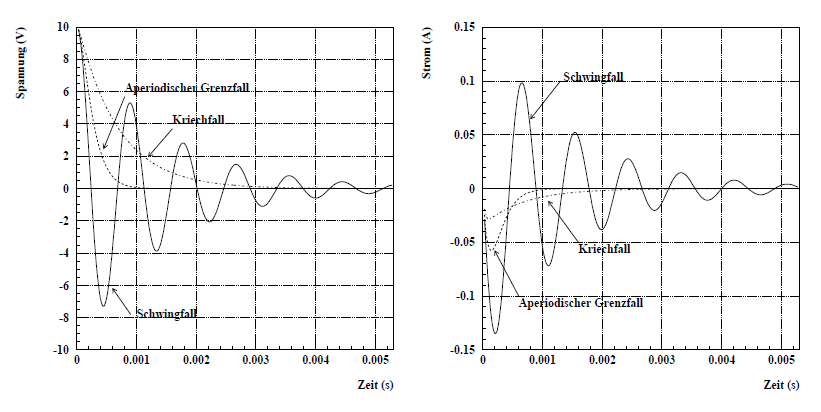
\includegraphics[scale=0.6]{Grundlagen.png}
\caption{Die drei Fälle beim Entladevorgang}
\label{Die drei Fälle beim Entladevorgang}
\end{figure}


\section{Aufbau und Durchführung}
\begin{figure}[H]
	\begin{minipage}{0.6\textwidth}
	Auf einer Rastersteckplatte werden die einzelnen Bauteile, wie in Abbildung \ref{Schaltplan}, eingesteckt und an einer Gleichspannungsquelle angeschlossen. Am Eingang A des Sensor- Cassy wird der Strom und am Eingang B die Spannung gemessen. Dabei muss im Menü des Cassy - Interface die richtigen Einstellungen(10 $\mu$s Messintervall, 20 ms Messzeit und 2000 Messungen) gewählt werden.	Der Kondensator wird durch die Spannungsquelle aufgeladen und anschließend wird der Taster betätigt, um die Spannungsquelle kurzzuschließen.  Der Ohmsche Widerstand wird variiert und die Messungen wiederholt. Die Widerstände, der Kondensator und die Spule werden vor dem Versuch mit einem Digitalvoltmeter vermessen. Mit dem Potentiometer wird der aperiodische Grenzfall bestimmt, indem zunächst der ungefähr benötigte Widerstand berechnet wird und dann das Potentiometer um diesen Wert reguliert wird, bis man einen Grenzfall beobachten kann. Dazu bestimmt man zuerst rechnerisch mit den obigen Formeln, wo ungefähr der aperiodische Grenzfall liegt.
	\end{minipage}
 	\hfill
	\begin{minipage}{0.3\textwidth}
	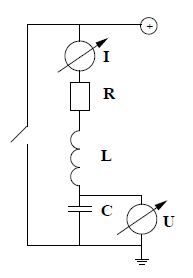
\includegraphics[scale=1]{Schaltplan.png}
	\caption{Schaltplan}
	\label{Schaltplan}
	\end{minipage}
\end{figure}

Beim Anschließen des Oszilloskops muss darauf geachtet werden, dass beide Channels den selben Ground haben. Für die Bestimmung der Dämpfungskonstante wird eine Schwingung mit \texttt{Single Sequence} aufgezeichnet, danach können die Peaks der Schwingung mit dem Cursor angefahren und Spannungs- und Zeit-Werte abgelesen werden.

\begin{figure}[H]
	\centering
	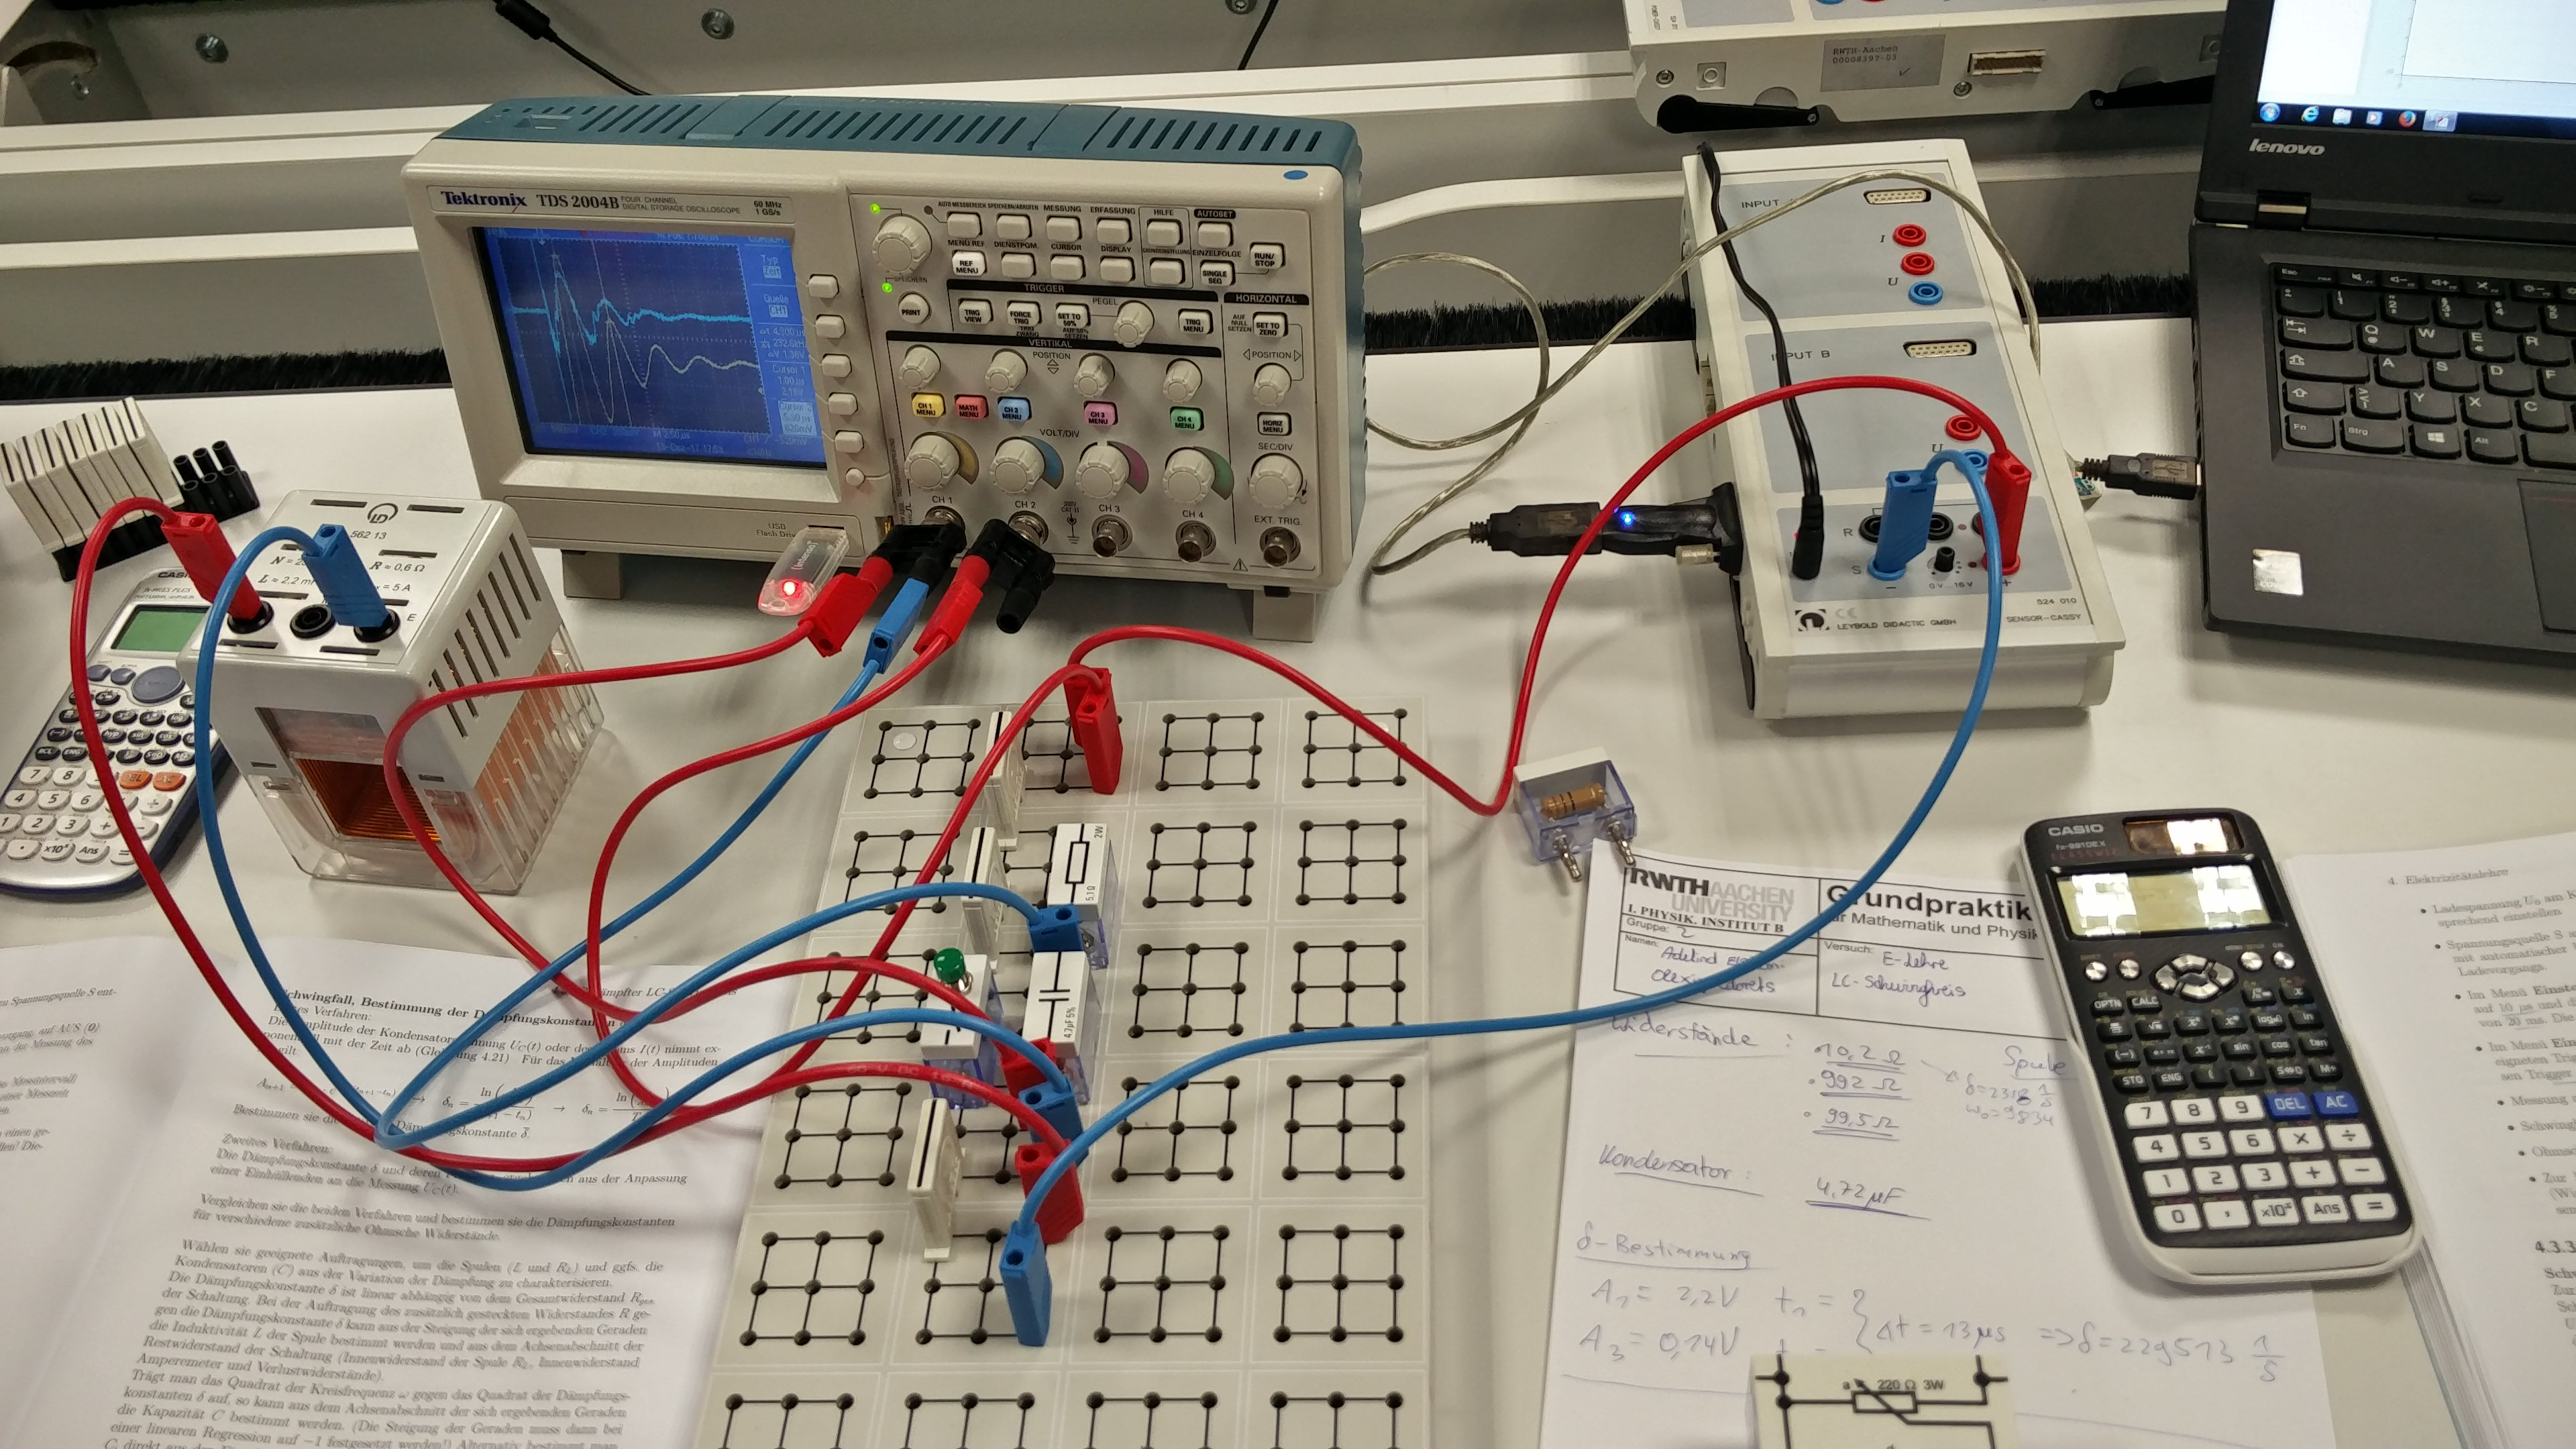
\includegraphics[scale=0.1]{../IMG_20171213_164200.jpg}
	\caption{Versuchsaufbau mit angeschlossenem Oszilloskop}
	\label{fig:Aufbau}
\end{figure}


\section{Auswertung}

\subsection{Bauteile}
Vor dem Versuch wurden zunächst alle Bauteile vermessen. Dafür wurde ein Digital-Multimeter verwendet, dessen Messfehler leider nicht bekannt war.


\begin{table}[H]
	\centering
	\renewcommand{\arraystretch}{1.2}
	\begin{tabular}{|c|c|c|c|c|c|}
		\hline 
		& Spule & Kondensator & \multicolumn{3}{|c|}{Widerstände} \\
		\hline
		Wert & $2.3 \;mH, 250 W., 0.7\;\Omega$ & $4.72 \;\mu F$ & $1.1 \Omega$ & $5.2 \Omega$ & $10.1 \Omega$ \\
		\hline
	\end{tabular}
	\label{table:Bauteile}
	\caption{Im Versuch verwendete Bauteile}
\end{table}

\subsection{Rohdaten}
Im Folgenden ist zu den drei oben genannten Fällen jeweils eine Beispielmessreihe zu sehen.

\paragraph{Schwingfall ($\delta < \omega_0$)} 1
     
\begin{figure}[H]
	\centering
	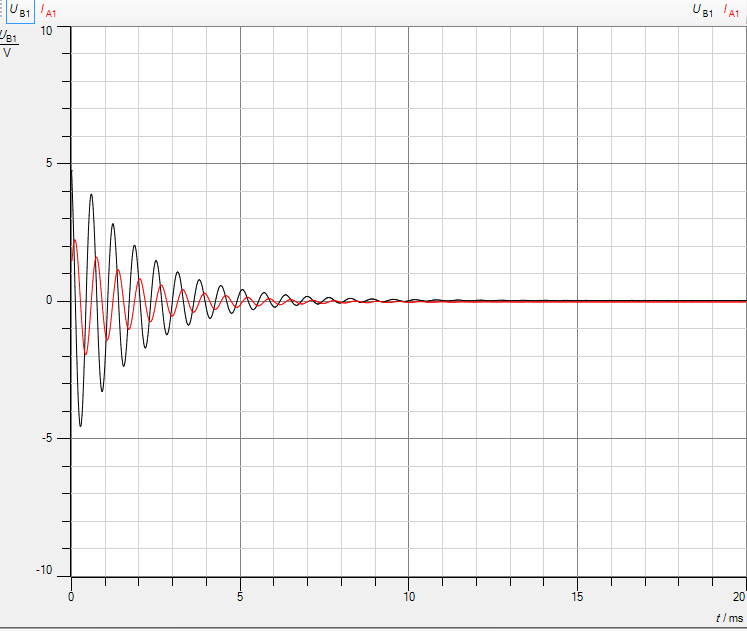
\includegraphics[scale=0.4]{1_Ohm-Schwingung.png}
	\caption{Schwingung bei einem Widerstand von 1 $\Omega$ (1. Messreihe)}
	\label{fig:Schwingung}
\end{figure}


\paragraph{Aperiodischer Grenzfall($\delta = \omega_0$)} 2
\begin{figure}[H]
	\centering
	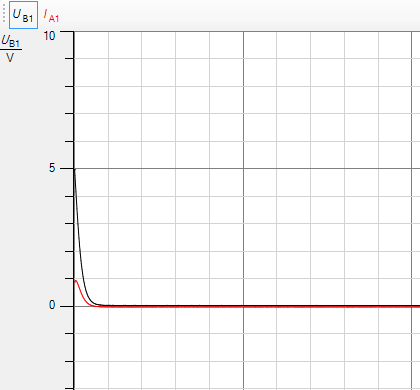
\includegraphics[scale=0.7]{Grenzfall.png}
	\caption{Grenzfall bei einem Widerstand von 43.27 $\Omega$ (1. Messreihe)}
	\label{fig:Grenzfall}
\end{figure}

\paragraph{Kriechfall ($\delta > \omega_0$)} 3	
\begin{figure}[H]
	\centering
	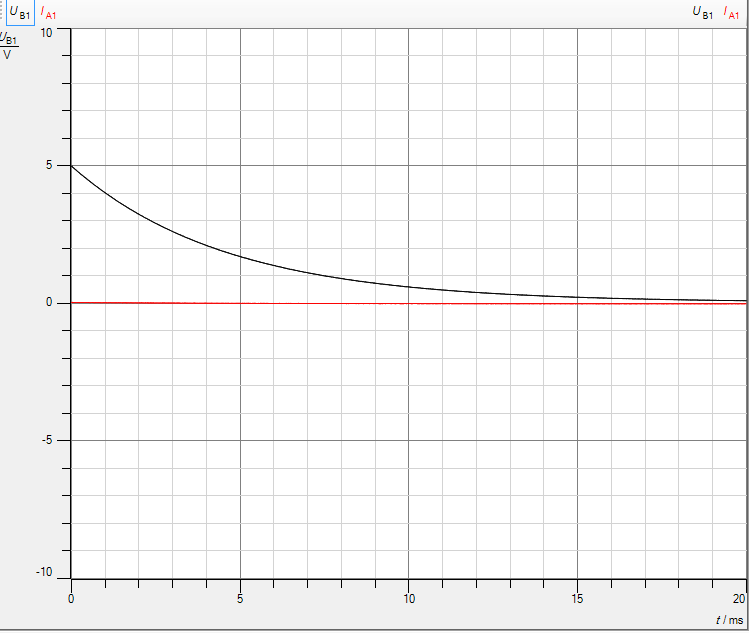
\includegraphics[scale=0.5]{Kriechfall.png}
	\caption{Kriechfall bei einem Widerstand von 1 $k\Omega$ (1. Messreihe)}
	\label{fig:Kriechfall}
\end{figure}


\subsection{Frequenzbestimmung}
Die Schwingunsfrequenz wurde mit verschiedenen Methoden jeweils für den Strom und die Spannung bestimmt. Die Ergebnisse waren sehr ähnlich, im Folgenden werden die Werte aus der Spannungsmessung verwendet.

\paragraph{Methode 1 - Nulldurchgänge} Es wurden die Nulldurchgänge der Schwingung und die Anzahl der Perioden gezählt, wobei der Ablesefehler der Abtastrate von $\sigma_t = 10 \mu s$ entspricht.
\begin{equation}
T = \frac{t_2 - t_1}{n} \quad \omega = \frac{2\pi}{T} \qquad \sigma_\omega = \omega \cdot \frac{\sqrt{2} \cdot \sigma_t }{n} \cdot \frac{1}{T}
\end{equation}
Da jeweils 3 Messungen für einen Widerstand gemacht wurden, werden die Frequenzen noch gewichtet gemittelt.

\paragraph{Methode 2 - FFT Peaks} In der FFT im CassyLab werden die Peaks bestimmt, wobei die Fehler auf die Peaks mit der Mehrfachmessung aus dem Fehler auf den Mittelwert bestimmt werden.

\begin{figure}[H]
	\centering
	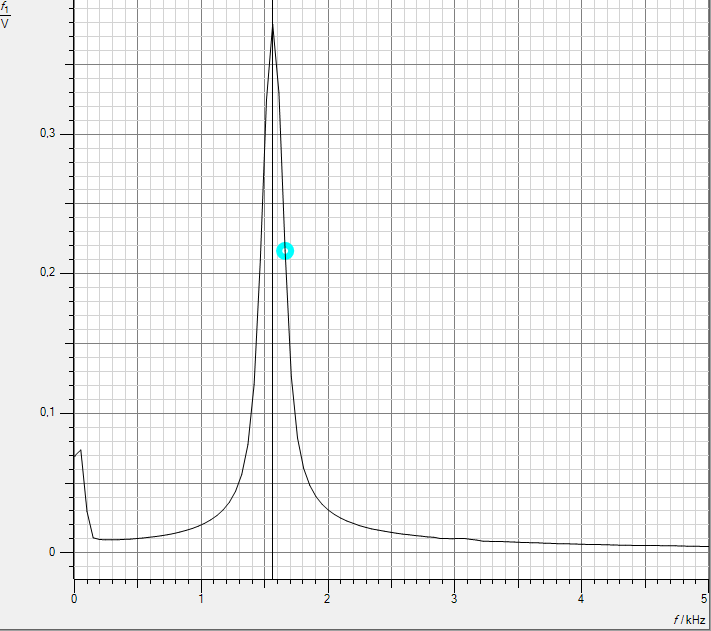
\includegraphics[scale=0.4]{Peakbestimmung.png}
	\caption{FFT der 1. Spannungsmessung bei 1$\Omega$, Peak bei $f=1563Hz$}
	\label{fig:fft}
\end{figure}

Die Ergebnisse der Frequenzbestimmung sind in Tabelle \ref{table:Frequenzen} zu sehen.

\begin{table}[H]
	\centering
	\renewcommand{\arraystretch}{1.2}
	\begin{tabular}{|c|c|c|c|c|}
		\hline 
		& $1.1 \Omega$ & $5.2 \Omega$ & $10.1 \Omega$ & $15.3 \Omega$ \\
		\hline 
		$\omega_{1} \;[1/s]$ & $10170 \pm 15$ & $9539 \pm 44$ & $9342 \pm 40$ & $8497 \pm 66$ \\
		\hline
		$\omega_{2} \;[1/s]$ & $9816 \pm 44$ & $ 10420 \pm 80$ & $ 10281 \pm 93$ & $10432 \pm 55$ \\
		\hline
	\end{tabular}
	\label{table:Frequenzen}
	\caption{Frequenzbestimmung durch Nulldurchgänge (1) und FFT-Peaks (2)}
\end{table}

\subsection{Bestimmung der Dämpfungskonstanten}
Die Dämpfungskonstanten wurden ebenfalls mit 2 Methoden bestimmt.
\paragraph{Methode 1 - Amplituden}
Aus dem Verhältnis der stetig abfallenden Amplituden kann mit folgender Formel die Dämpfungskonstante ermittelt werden:
\begin{equation}\label{eq:delta}
\delta_n = \frac{\ln \left(A_n/A_{n+1}\right)}{t_{n+1}-t_n}
\end{equation}

\paragraph{Methode 2 - Einhüllende}
Mit Hilfe des CassyLaby wurde eine exponentielle Einhüllende an die Schwingung gelegt, was Beispielhaft in Abbildung \ref{fig:einhuellende} zu sehen ist.
Daraus erhält man die Dämpfungskonstante.
\begin{figure}[H]
	\centering
	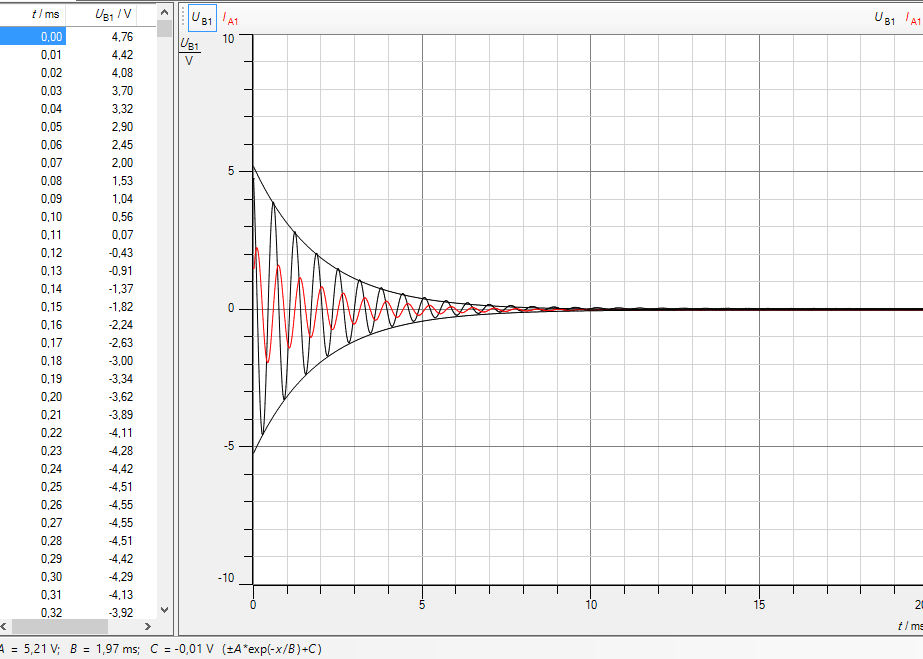
\includegraphics[scale=0.5]{EinhuellendemitWerte.png}
	\caption{exp()-Einhüllende der 1. Spannungsmessung bei 1$\Omega$, $\delta = 510 \;1/s$}
	\label{fig:einhuellende}
\end{figure}
Leider konnte mit dieser Methode das $\delta$ bei einem Widerstand von $15\Omega$ nicht bestimmt werden, da es dort nur eine Schwingung gab und keine Einhüllende gelegt wurde.

Die so bestimmten Dämpfungskonstanten aus mehreren Messungen wurden jeweils untereinander gemittelt und der Fehler auf den Mittelwert bestimmt.
Diese Ergebnisse sind in Tabelle \ref{table:deltas}

\begin{table}[H]
	\centering
	\renewcommand{\arraystretch}{1.2}
	\begin{tabular}{|c|c|c|c|c|}
		\hline 
		& $1.1 \Omega$ & $5.2 \Omega$ & $10.1 \Omega$ & $15.3 \Omega$ \\
		\hline 
		$\delta_{1} \;[1/s]$ & $567 \pm 10$ & $1403 \pm 11$ & $2323 \pm 63$ & $2657 \pm 199$ \\
		\hline
		$\delta_{2} \;[1/s]$ & $520 \pm 8$ & $ 1470 \pm 82$ & $ 2520 \pm 16$ & - \\
		\hline
		$\delta_{theo} \;[1/s]$ & $239$ & $1130$ & $ 2196$ & $3326$ \\
		\hline
	\end{tabular}
	\label{table:deltas}
	\caption{$\delta$-Bestimmung durch Amplituden und Einhüllende}
\end{table}

\subsubsection{$\delta$-Bestimmung mit dem Oszilloskop}
Zusätzlich wurde während des Versuchs die Dämpfungskonstante für den $5.2\,\Omega$-Widerstand mit dem Oszilloskop bestimmt.
\begin{figure}[H]
	\centering
	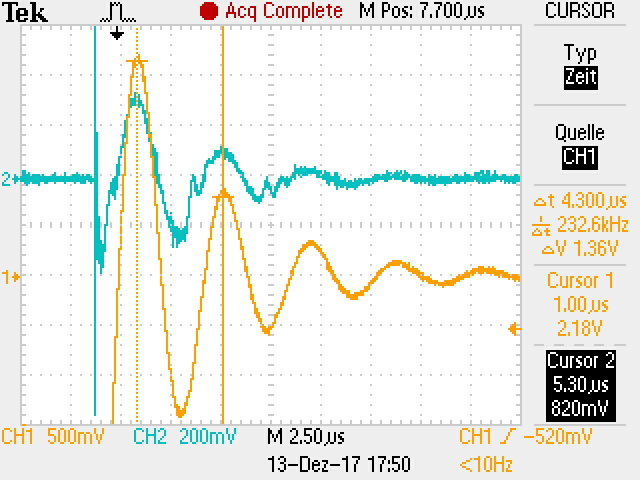
\includegraphics[scale=1]{../Oszi/F0008TEK.JPG}
	\caption{$\delta$-Bestimmung mit dem Oszilloskop}
	\label{fig:Oszi}
\end{figure}

Mit dem Cursor wurden folgende Werte abgelesen: $A_1 = 3.04V, \;A_2 = 1.08V, \;\Delta t = 640\,\mu s$. Mit der Formel \ref{eq:delta} ergibt sich eine Dämpfungskonstante von $\delta = 1617 \, 1/s$.



\subsection{Charakterisierung der Spule}\label{sec:Spule}
Zur Bestimmung der Induktivität und des Spulenwiderstands wurde für beide Methoden der $\delta$-Bestimmung jeweils eine lineare Regression mit $f(x)=a \cdot x+b$ durchgeführt. Diese sind in den Abbildungen \ref{fig:Spule1} und \ref{fig:Spule2} zu sehen.
Bei der Auftragung von $\delta$ gegen R gelten folgende Zusammenhänge
\begin{equation}
\delta = \frac{R+R_{rest}}{2L} \quad \Rightarrow \quad a = \frac{1}{2L}, \; b = \frac{R_{rest}}{2L} \quad \Rightarrow \quad L = \frac{1}{2a}, \; R_{rest} = \frac{b}{a}
\end{equation}
Damit Ergeben sich die in Tabelle \ref{table:SpuleRL} zu sehenden Werte. Diese sind mit den realen Werten in Tabelle \ref{table:Bauteile} verglichen.

\begin{table}[H]
	\centering
	\renewcommand{\arraystretch}{1.2}
	\begin{tabular}{|c|c|c|c|c|}
		\hline 
		& Methode 1 & Methode 2 & Sollwert & Abweichung\\
		\hline 
		a [1/H] & $199.9 \pm 9.4$ & $222.3 \pm 0.9$ &  &\\
		\hline
		b [$\Omega$/H] & $353 \pm 35.5$ & $ 275.7 \pm 4.4$  & &\\
		\hline
		$\chi^2/ndf$ & $8.4$ & $0.2$ &  &\\
		\hline
		L [mH] & $2.50 \pm 0.12$ & $2.25 \pm 0.01$ & 2.3 & $1.6 \sigma (1), \; 5\sigma (2)$ \\
		\hline
		$R_{rest} \,[\Omega]$ & $1.76 \pm 0.20$ & $1.24 \pm 0.02$ & 0.7 & $5.3\sigma(1), \; 27\sigma(2) $ \\
		\hline
	\end{tabular}
	\label{table:SpuleRL}
	\caption{Bestimmung der Induktivität und des Restwiderstands}
\end{table}

Der hier als $R_{rest}$ bestimmte Widerstand bezeichnet den gesamten restlichen Widerstand, der sowohl den Innenwiderstand der Spule $R_L$ als auch den Innenwiderstand des Amperemeters  und Verlustwiderstände durch Drähte etc. beinhaltet. Das erklärt die Abweichungen von dem erwarteten Wert von $R_L = 0.7 \Omega$.

Die zweite Methode der $\delta$-Bestimmung liefert sehr geringe Fehler, was sich auch im $\chi^2/ndf$ widerspiegelt. Hier fällt der sehr große Fehler vom Wert bei 5.2 $\Omega$ auf. Bei der ersten Methode ist das $\chi^2/ndf$ von 8 zu hoch, da der letzte Wert bei 15.3 $\Omega$ verglichen mit den anderen ein Ausreißer ist.


%[ 199.90097428  352.75837857] [  9.41723794  35.54705826] 8.39768478359
%L1 = 2.501 \pm 0.118 mH
%RL1 = 1.765 \pm 0.196 Ohm
%[ 222.27610929  275.70292495] [ 0.9530111   4.41012641] 0.221405548694
%L2 = 2.249 \pm 0.010 mH
%RL2 = 1.240 \pm 0.021

\begin{figure}[H]
	\centering
	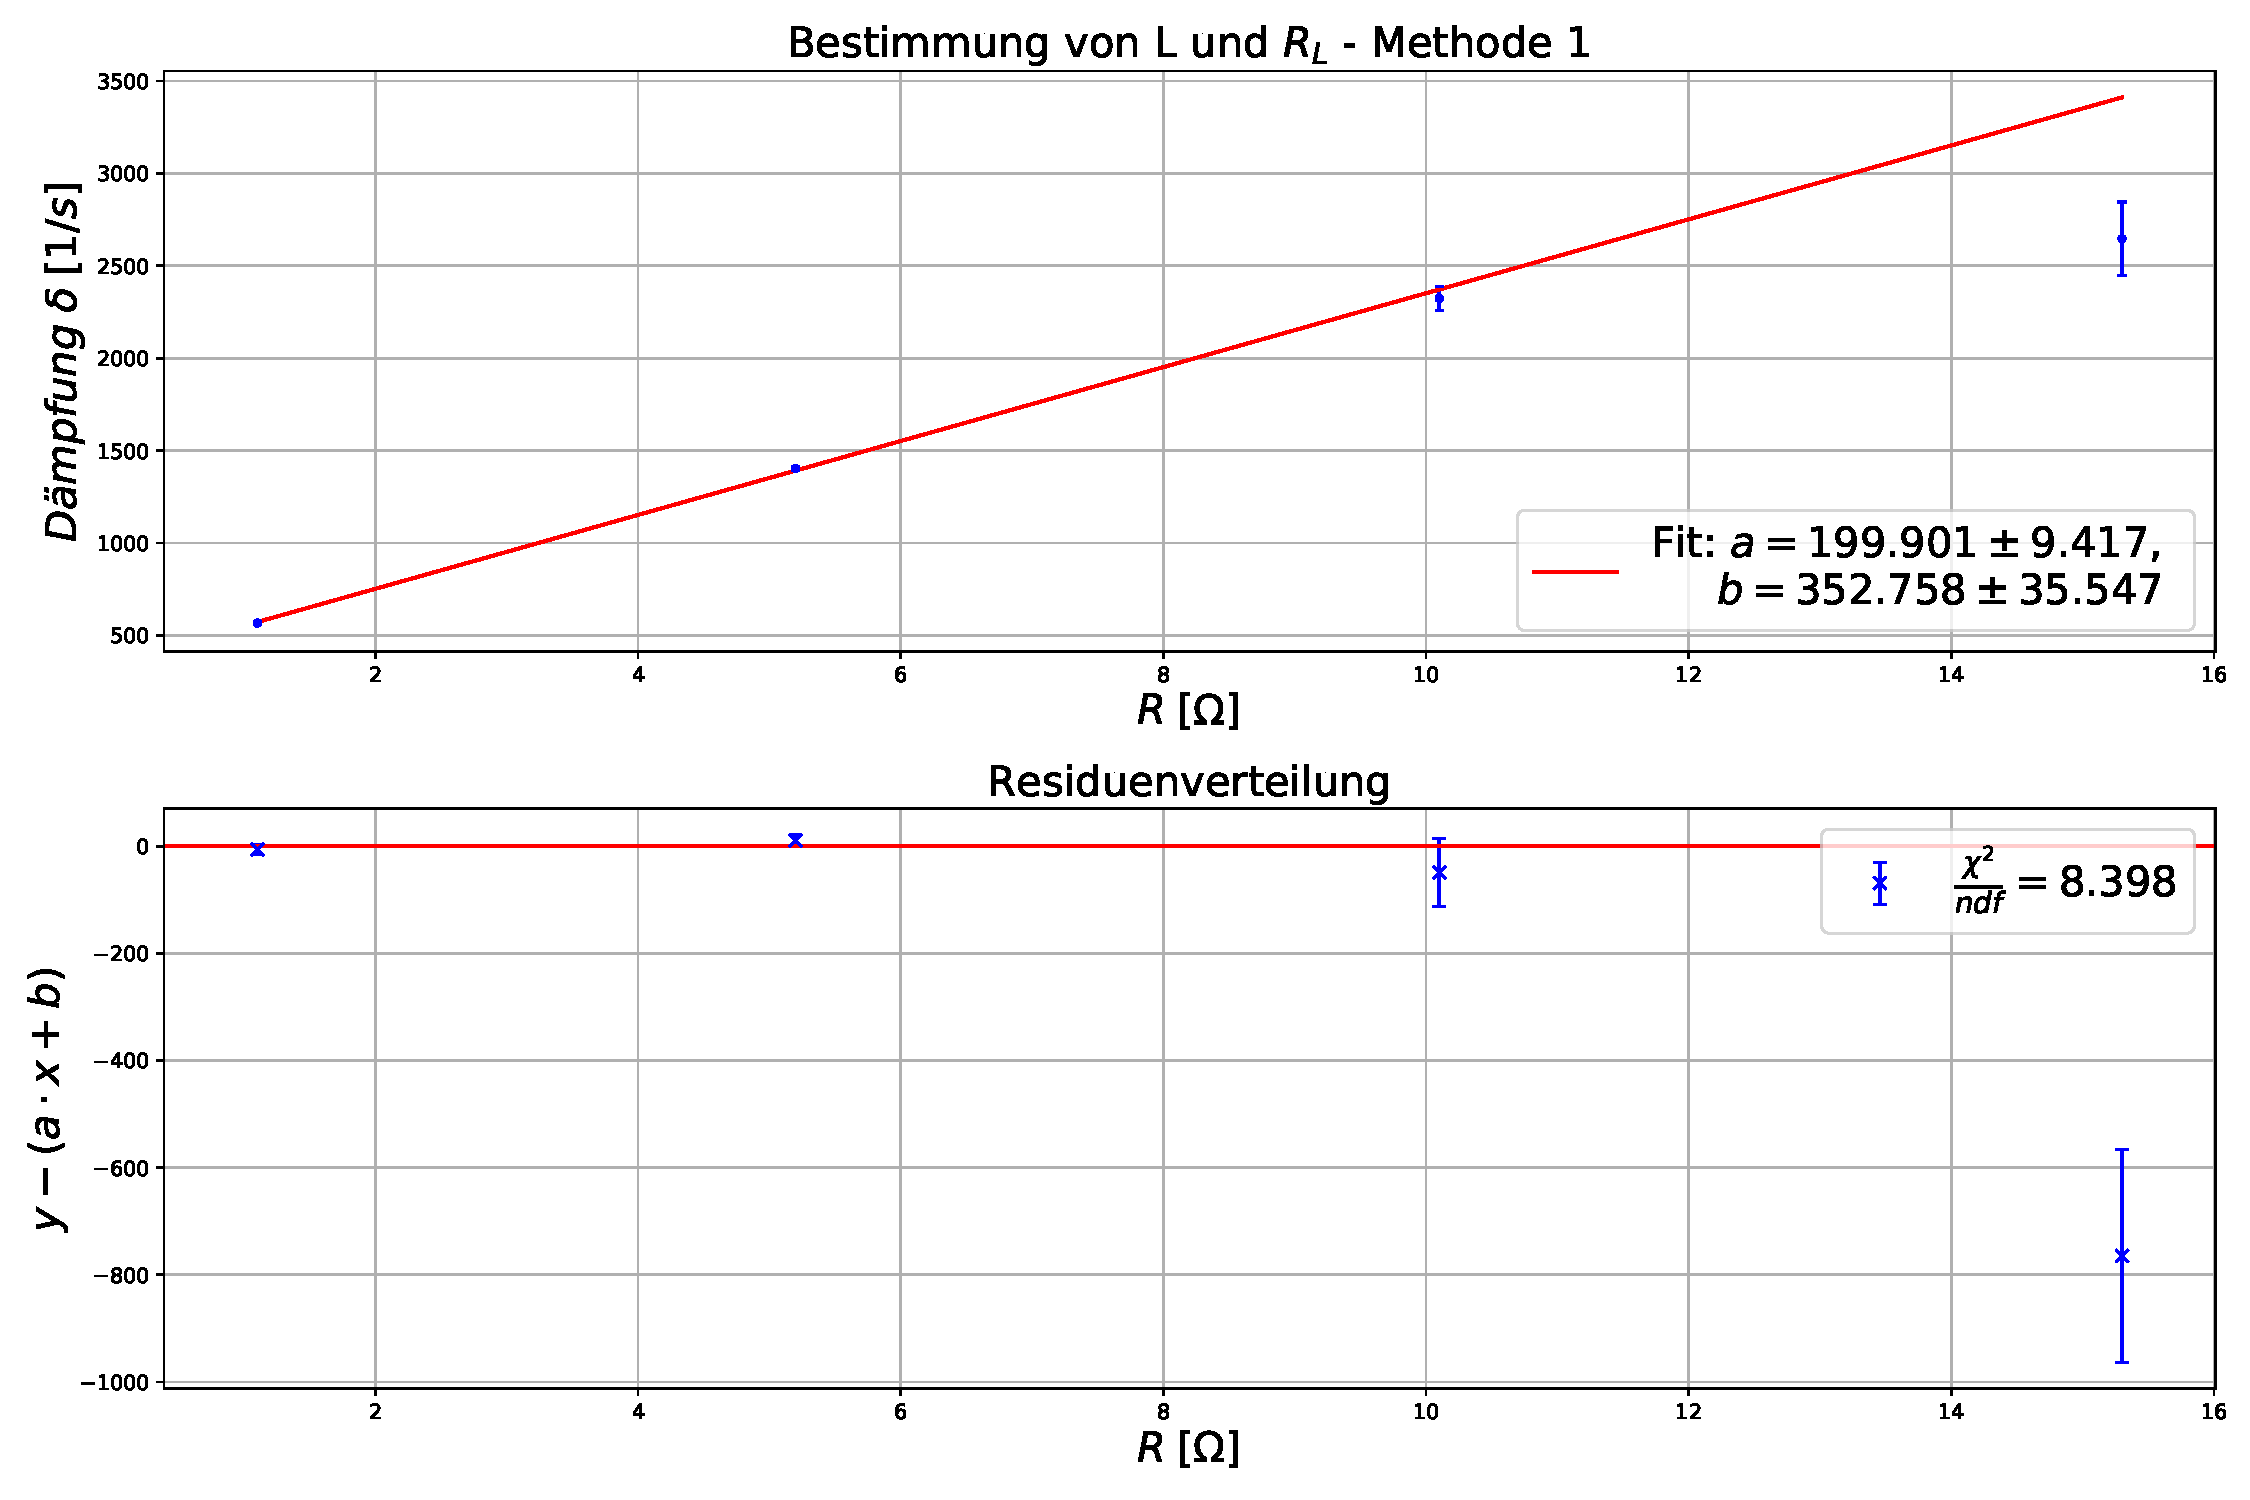
\includegraphics[scale=0.4]{../Plots/BestimmungLR_LMethode1.pdf}
	\caption{lineare Regression von $\delta$ gegen R mit Dämpfungen nach Methode 1}
	\label{fig:Spule1}
\end{figure}

\begin{figure}[H]
	\centering
	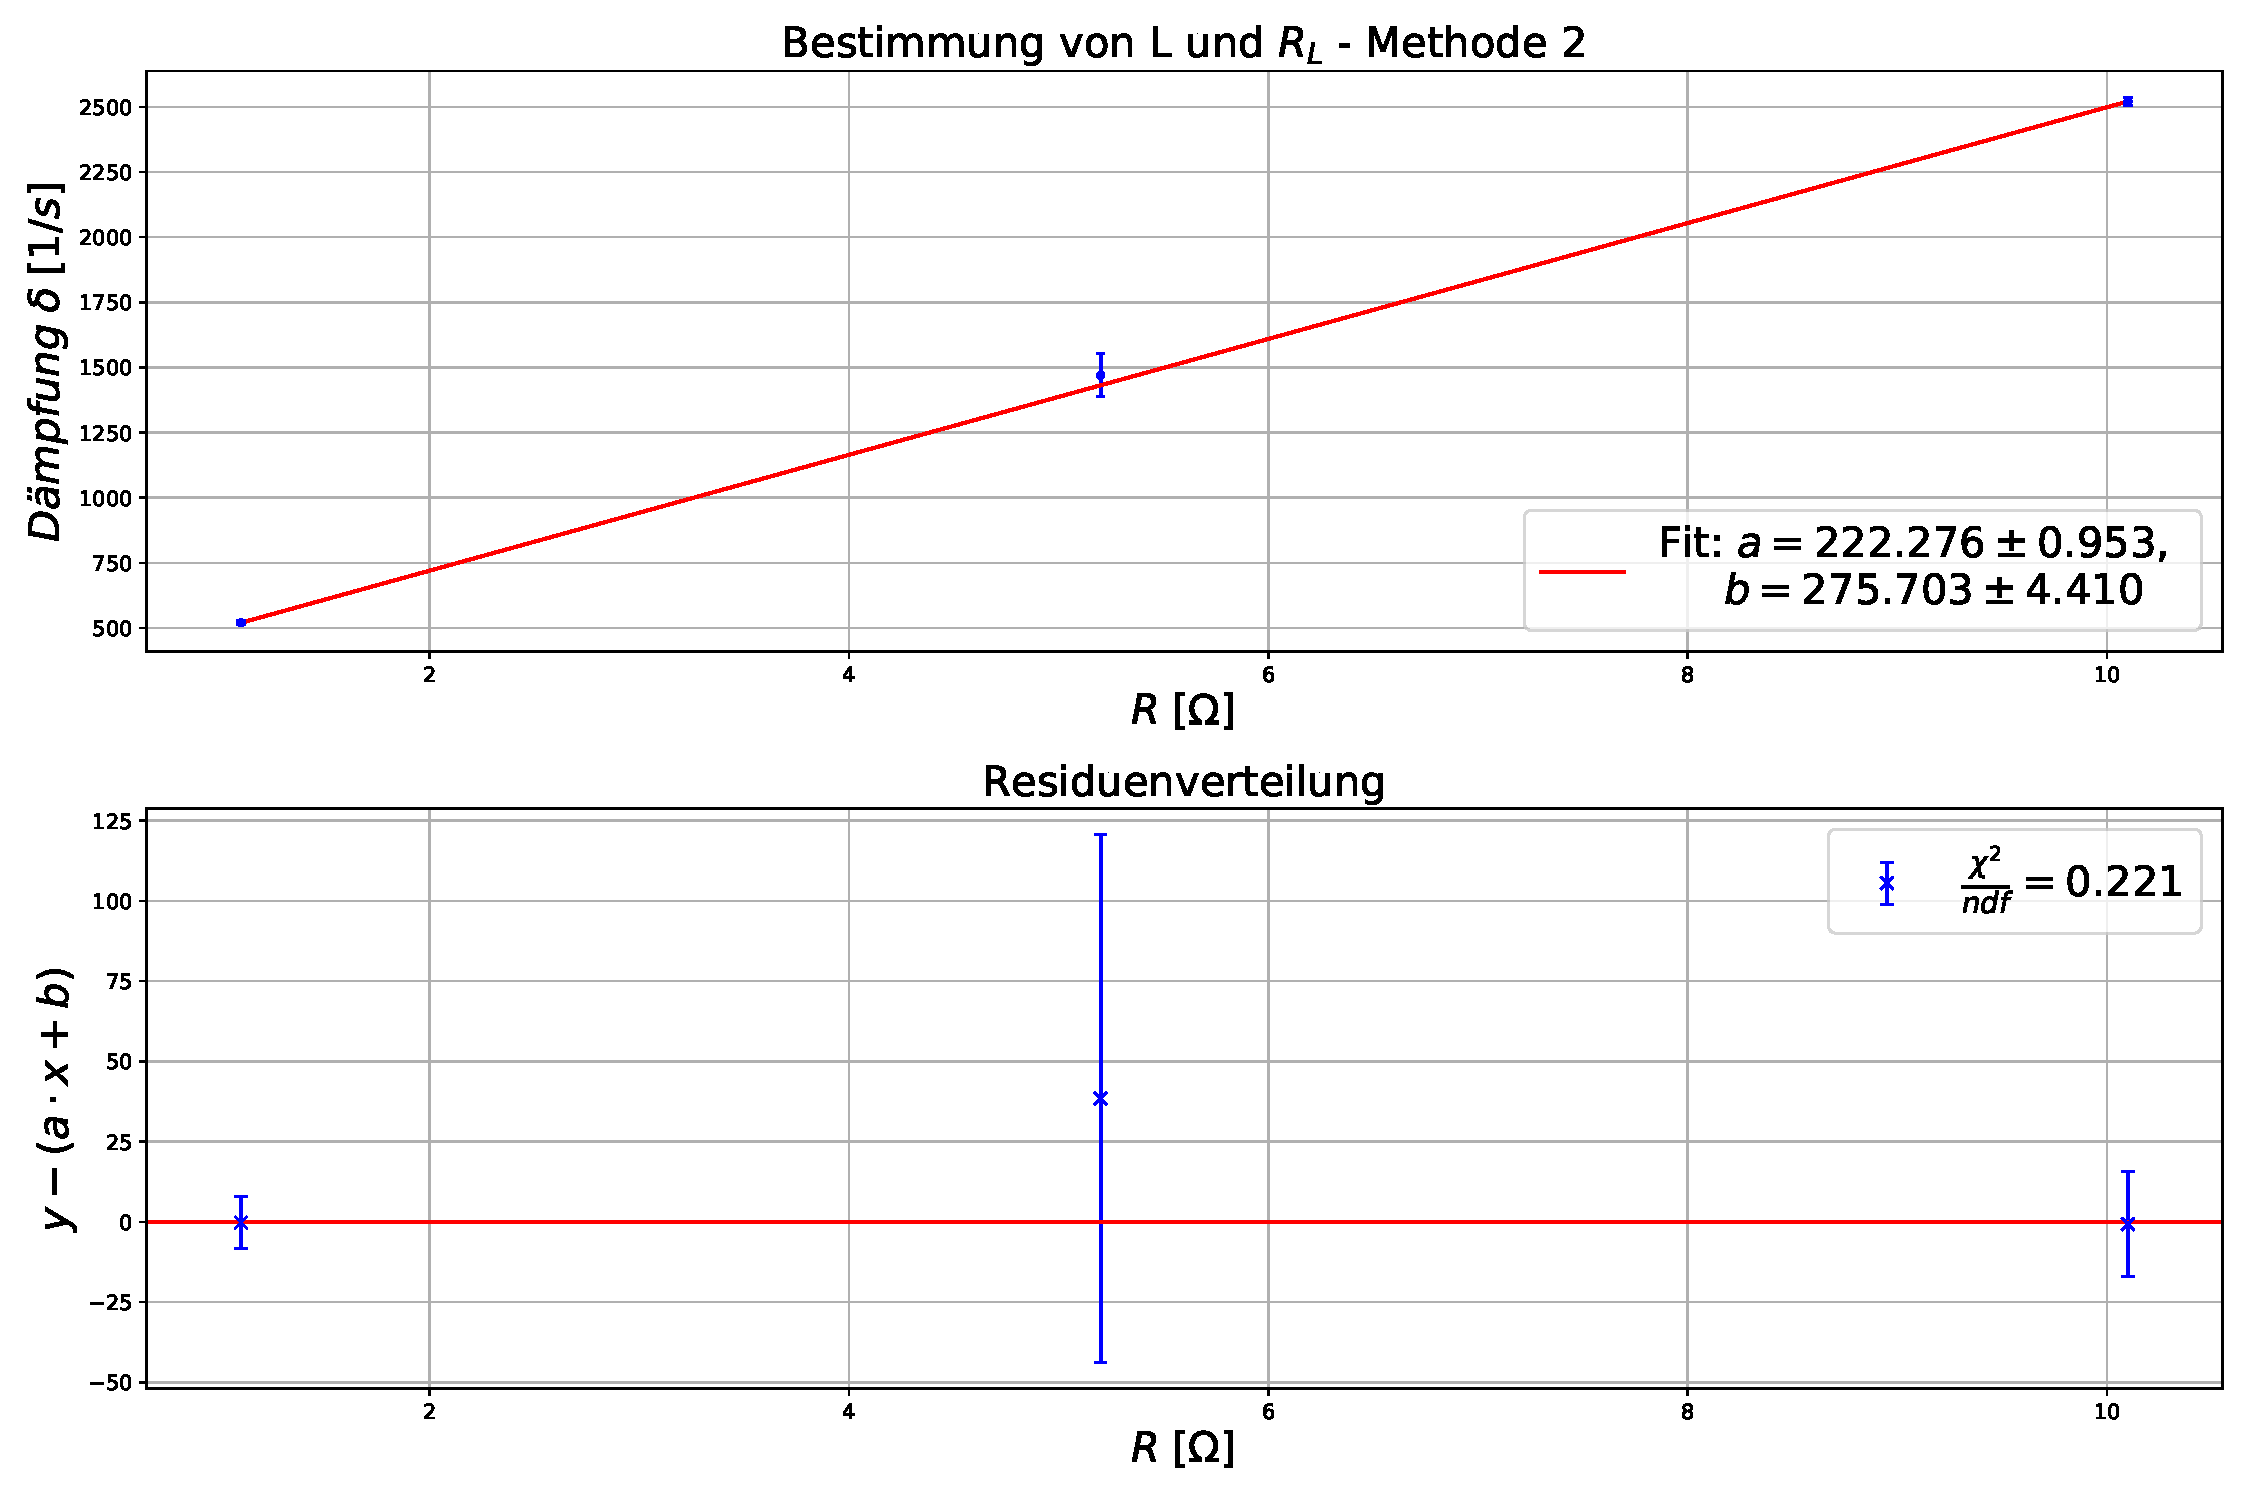
\includegraphics[scale=0.4]{../Plots/BestimmungLR_LMethode2.pdf}
	\caption{lineare Regression von $\delta$ gegen R mit Dämpfungen nach Methode 2}
	\label{fig:Spule2}
\end{figure}


\subsection{Charakterisierung des Kondensators}
Um die Kapazität des Kondensators zu bestimmen wurde bei der linearen Regression $\omega^2$ gegen $\delta^2$ aufgetragen und die Steigung der Geraden auf -1 festgelegt. Durch die Kombination der verschiedenen Auswertemethoden bei der Bestimmung von Frequenz und Dämpfungskonstante ergaben sich die folgenden 4 Regressionen.

\begin{figure}[H]
	\centering
	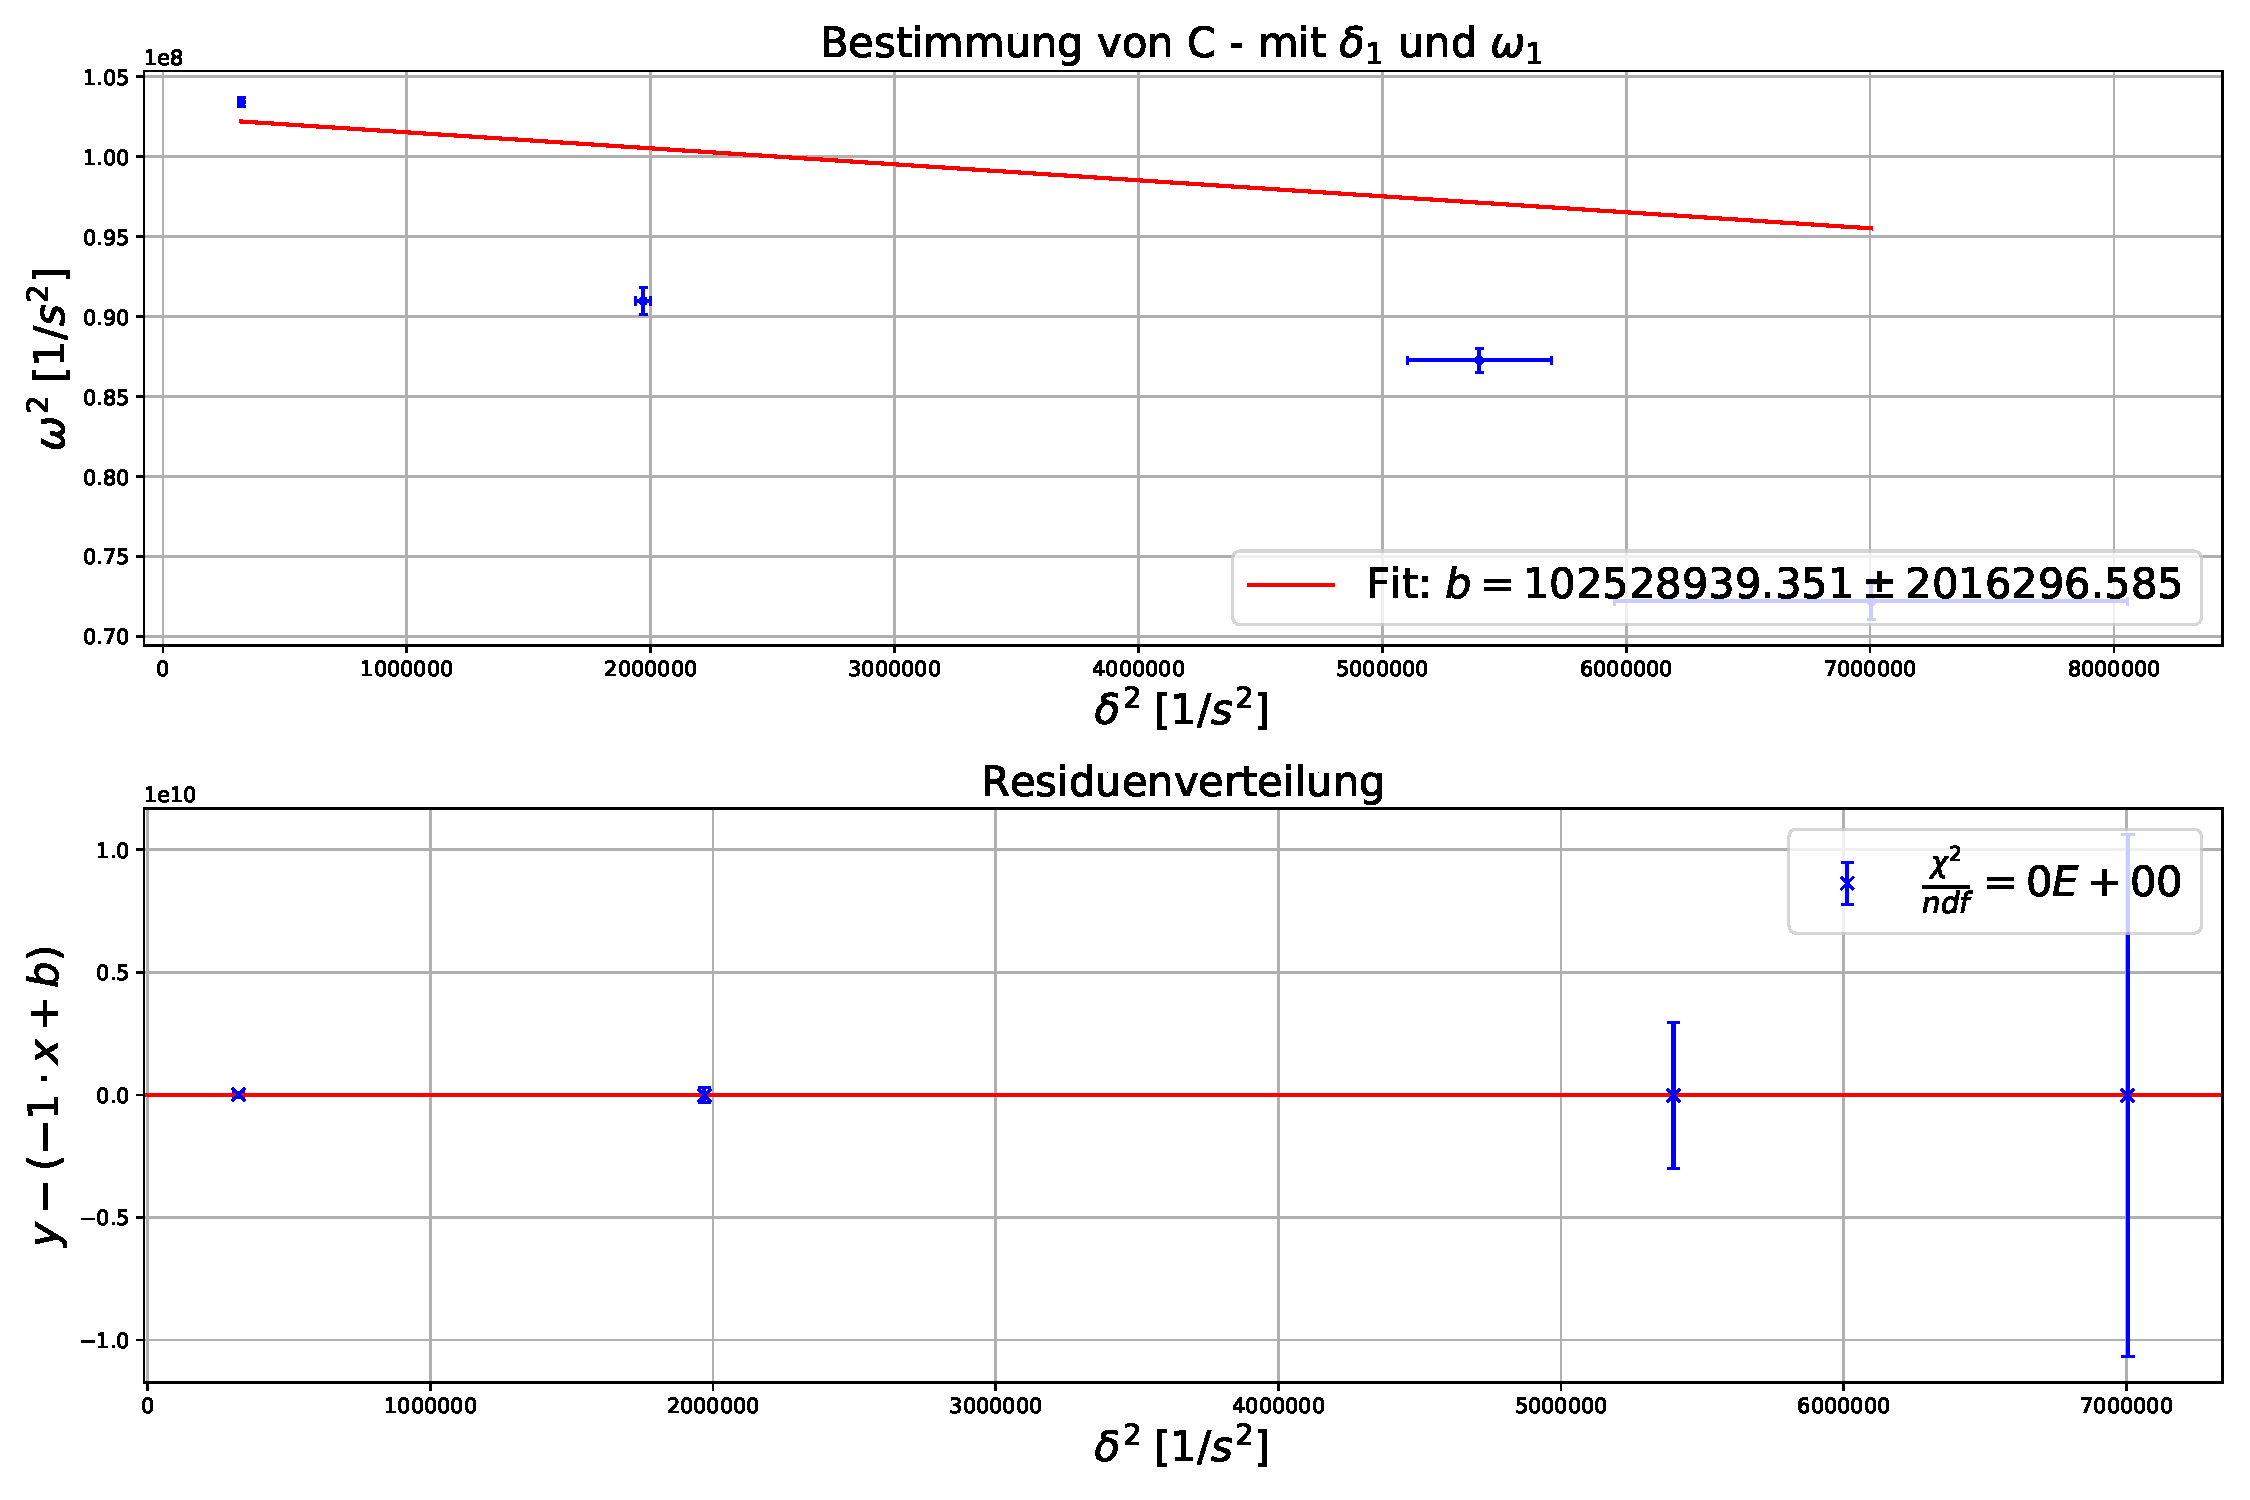
\includegraphics[scale=0.4]{../Plots/BestimmungCdelta_1omega_1.pdf}
	\caption{Bestimmung der Kapazität mit $\delta$ und $\omega$ nach Methode 1}
	\label{fig:C11}
\end{figure}

\begin{figure}[H]
	\centering
	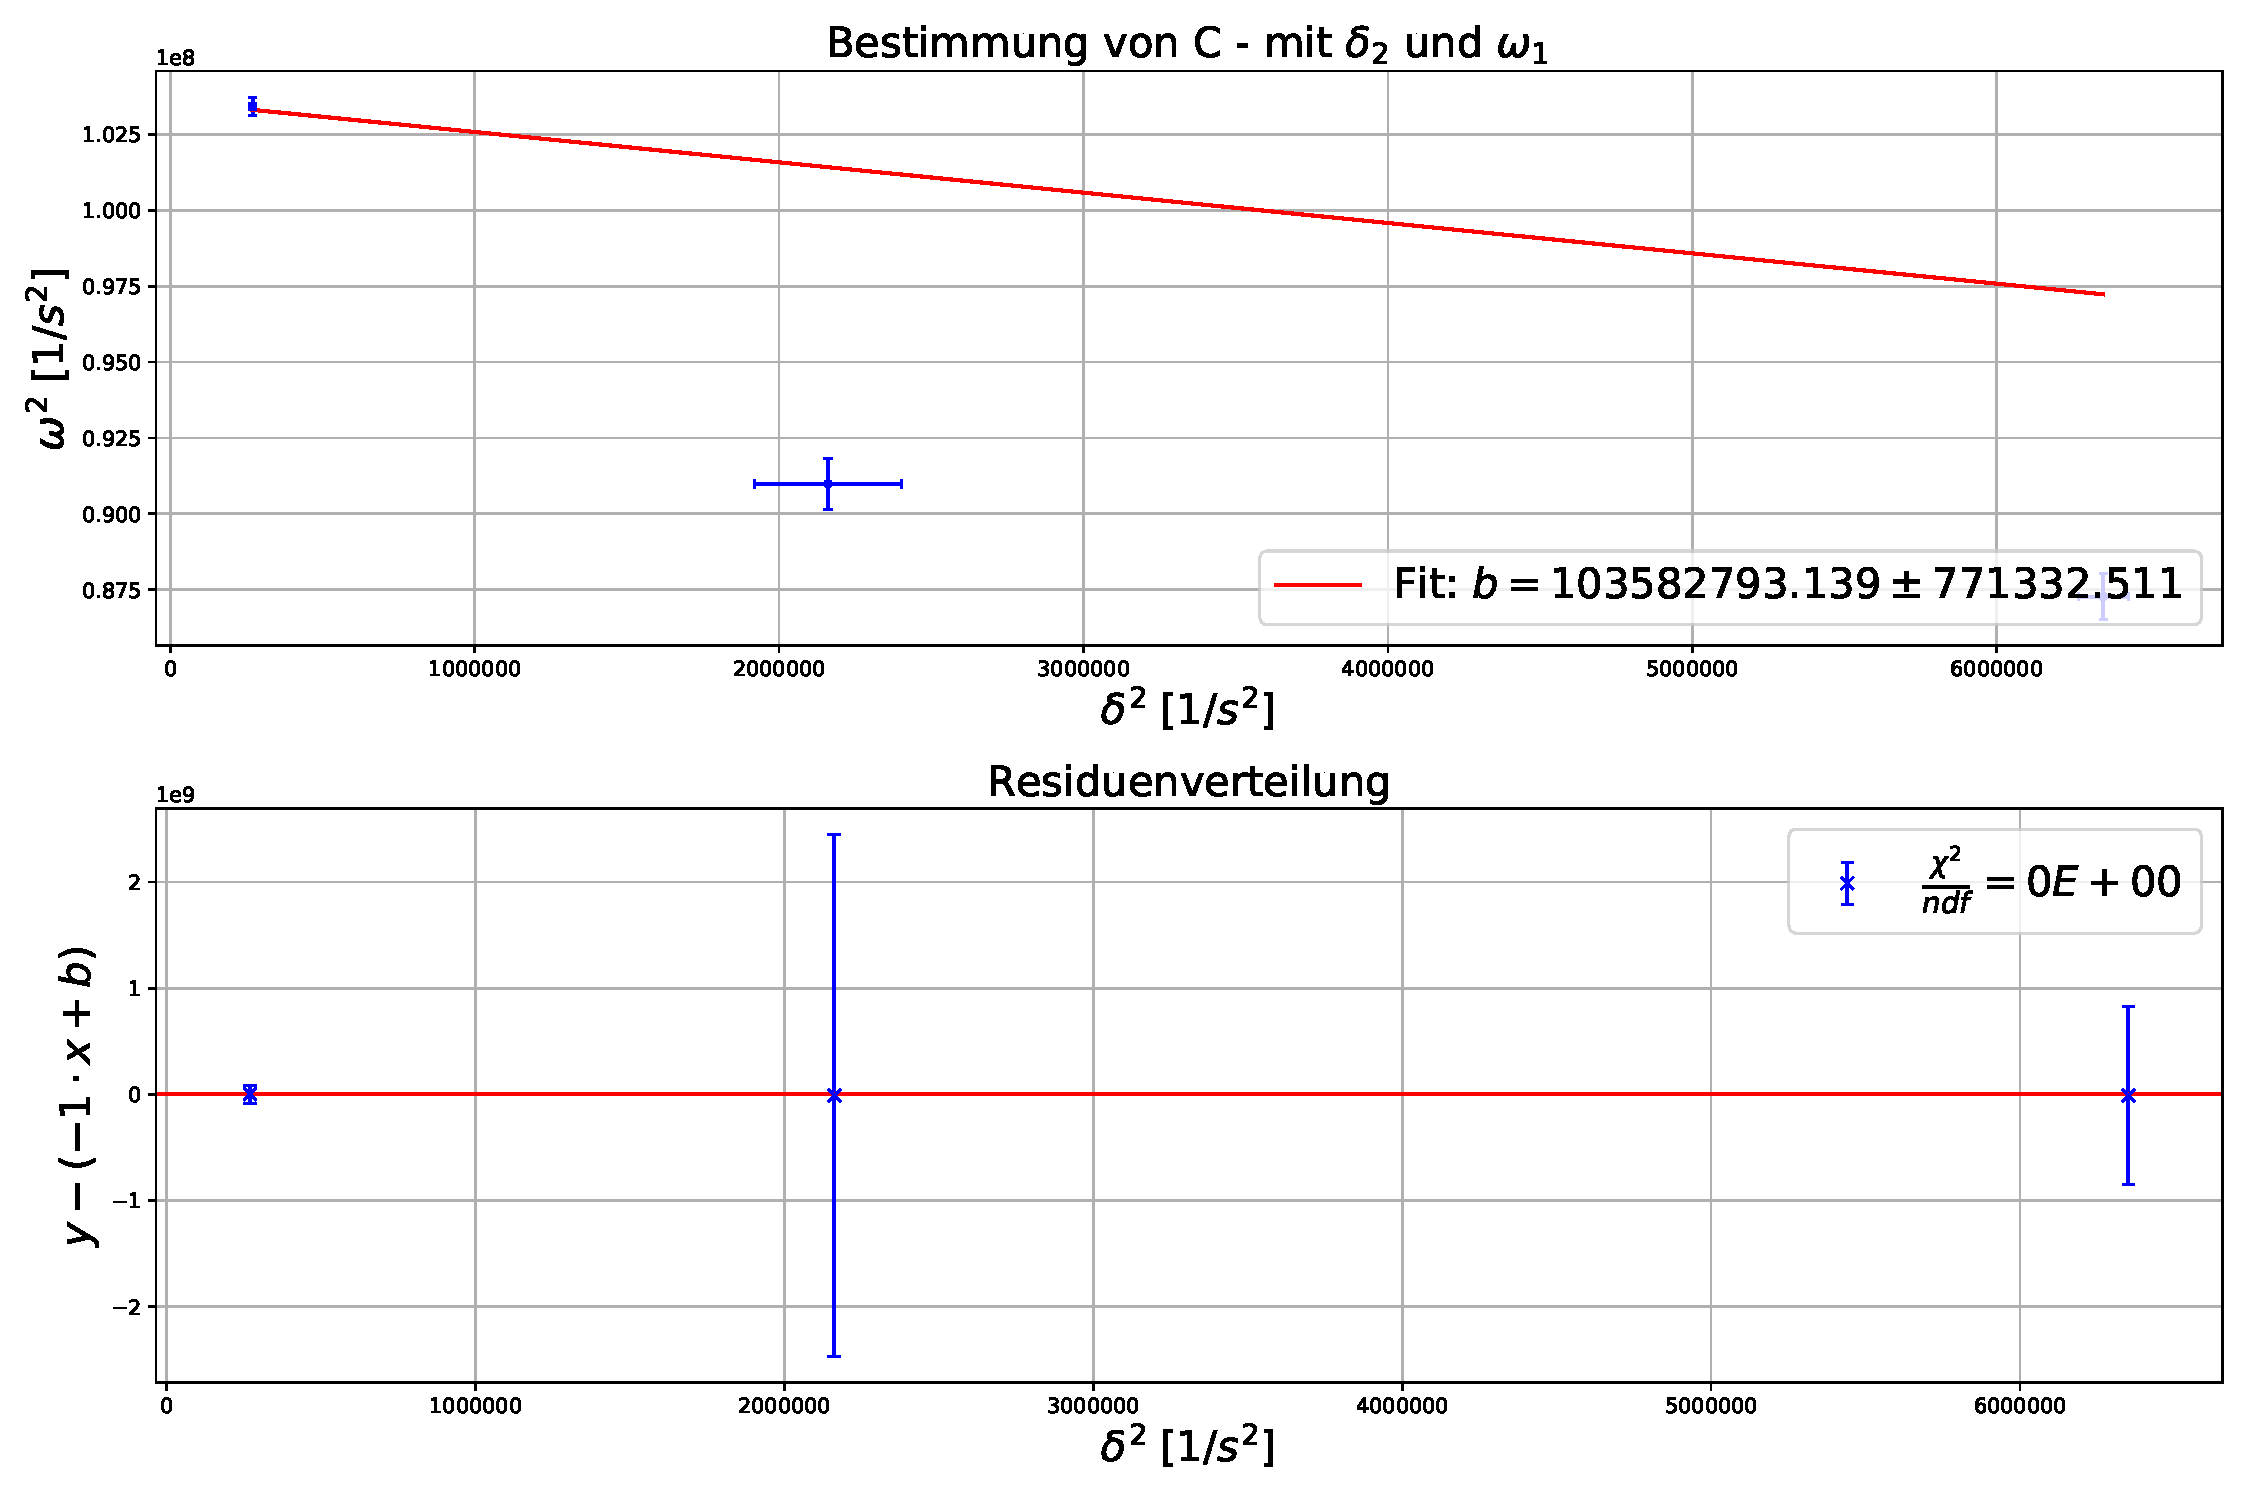
\includegraphics[scale=0.4]{../Plots/BestimmungCdelta_2omega_1.pdf}
	\caption{Bestimmung der Kapazität mit $\delta$ nach Methode 2 und $\omega$ nach Methode 1}
	\label{fig:C21}
\end{figure}

\begin{figure}[H]
	\centering
	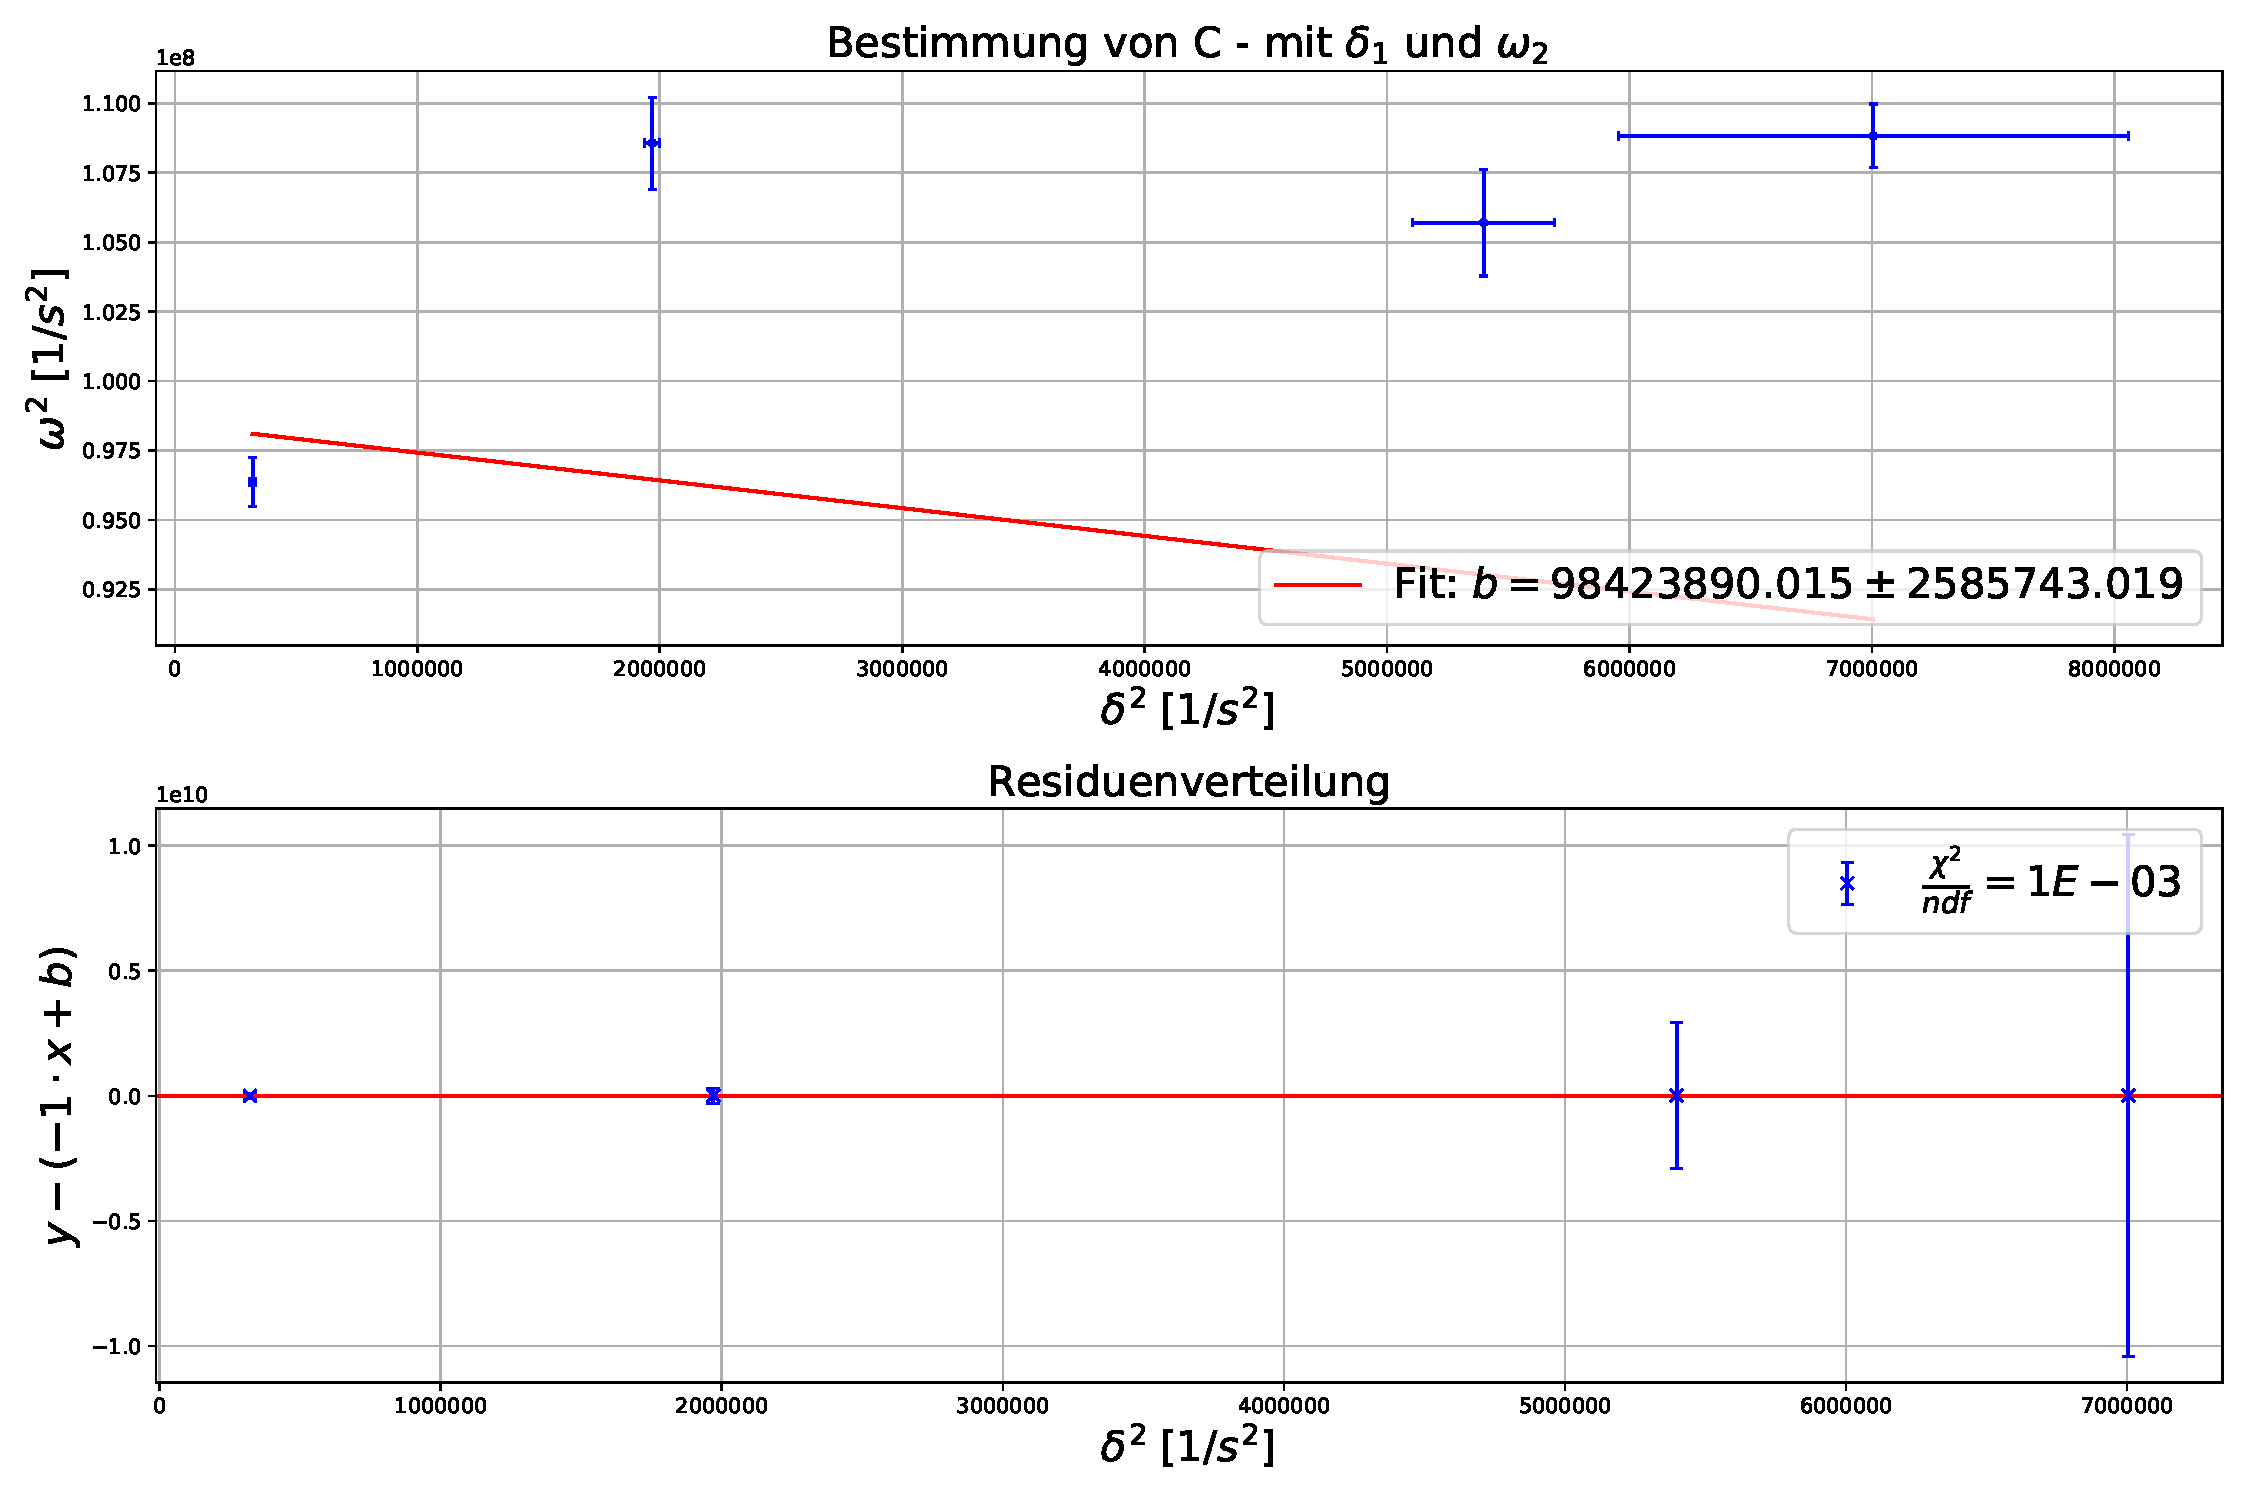
\includegraphics[scale=0.4]{../Plots/BestimmungCdelta_1omega_2.pdf}
	\caption{Bestimmung der Kapazität mit $\delta$ nach Methode 1 und $\omega$ nach Methode 2}
	\label{fig:C12}
\end{figure}

\begin{figure}[H]
	\centering
	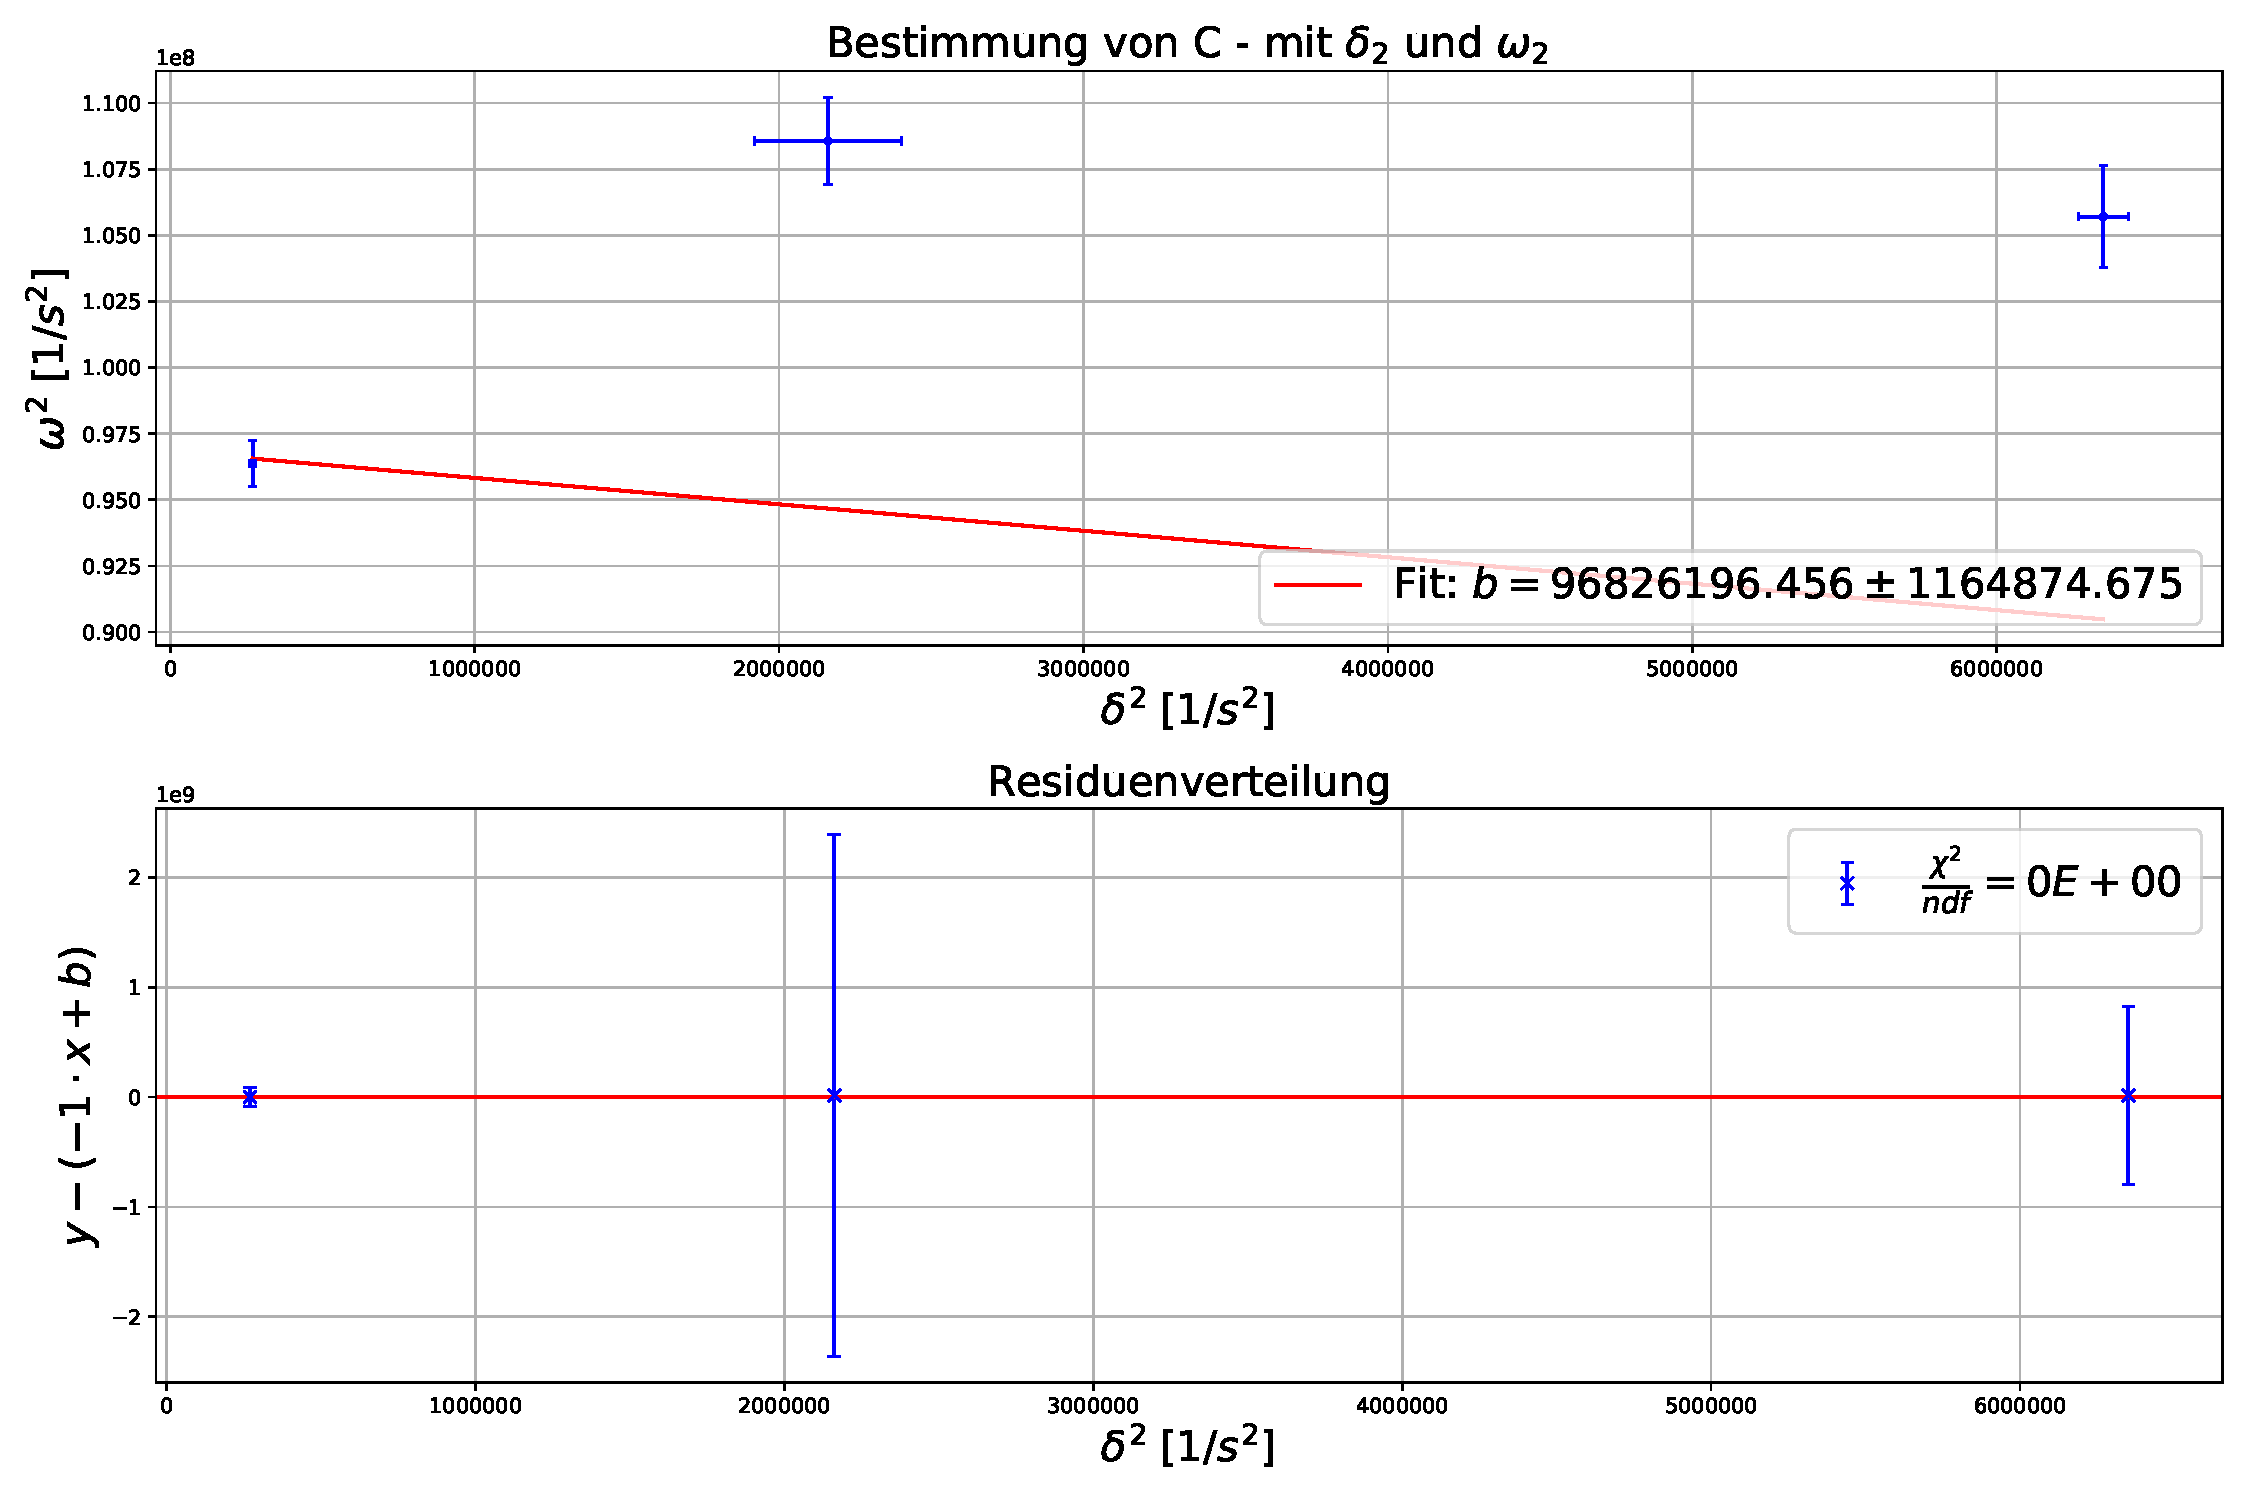
\includegraphics[scale=0.4]{../Plots/BestimmungCdelta_2omega_2.pdf}
	\caption{Bestimmung der Kapazität mit $\delta$ und $\omega$ nach Methode 2}
	\label{fig:C22}
\end{figure}

Mit Hilfe der Zusammenhänge
\begin{equation}
L = \frac{1}{\omega^2C + \delta^2C} \quad \Rightarrow \quad \omega^2 = -\delta^2 + \frac{1}{LC} \quad \Rightarrow \quad C = \frac{1}{L \cdot b},\; \sigma_C = C \cdot \sqrt{\left(\frac{\sigma_L}{L}\right)^2 + \left(\frac{\sigma_b}{b}\right)^2} 
\end{equation}
erhält man daraus die in Tabelle \ref{table:KondensatorC} gezeigten Kapazitäten.

\begin{table}[H]
	\centering
	\renewcommand{\arraystretch}{1.2}
	\begin{tabular}{|c|c|c|c|c|}
		\hline 
		& $\delta_{1},\omega_{1}$ & $\delta_{2},\omega_{1}$ & $\delta_{1},\omega_{2}$ & $\delta_{2},\omega_{2}$\\
		\hline 
		C [$\mu F$] & $4.34 \pm 0.09$ & $4.29 \pm 0.04$ & $4.52 \pm 0.12$ & $4.59 \pm 0.06$\\
		\hline
		Abweichung von $4.72 \;\mu F$ & $4.2\;\sigma$ & $11\;\sigma$ & $1.7\;\sigma$ & $2.2\;\sigma$ \\
		\hline
	\end{tabular}
	\label{table:KondensatorC}
	\caption{Bestimmung der Kapazität des Kondensators (hier steht der Index für die Methode der $\delta$- bzw. $\omega$-Bestimmung, dessen Daten für die lineare Regression verwendet wurden)}
\end{table}

Dabei fällt auf, dass die Verwendung der Frequenzdaten aus der FFT-Peakbestimmung wesentlich bessere Ergebnisse für die Kapazität liefert.

Trotz der scheinbar sehr schlechten Fits ließ sich hier die Kapazität dennoch gut abschätzen.

\subsection{Aperiodischer Grenzfall}
Zusätzlich wird der Widerstand bestimmt, der für einen aperiodischen Grenzfall benötigt bzw. gesteckt werden muss. 
\begin{equation}
R_{ges} = R_{ap} + R_{rest} = 2 \cdot \sqrt{\frac{L}{C}}
\end{equation}
Rechnerisch ergab sich dieser während des Versuchs zu $R_{ap} = 44.15 \;\Omega$, mit dem in Abschnitt \ref{sec:Spule} bestimmten Wert für $R_{rest} = 1.25\;\Omega$ (hierfür wurde gewichtet gemittelt) ergibt sich eine Erwartung von $R_{ap} = 42.9 \;\Omega$. Bei einer Einstellung des Potentiometers von $43.27 \;\Omega$ wurde dann der Grenzfall beobachtet, der bereits in Abbildung \ref{fig:Grenzfall} gezeigt wurde. 


\section{Fazit}

\clearpage
\listoffigures
\listoftables

\end{document}

